% ../../../1994_全国卷_理科/figures/f1994_national_science_q23_prism.tex — 1994 年·全国卷·理科 第 23 题（棱柱）
%
% 【来源】`.work/phase4-b19/source/1994全国理.pdf`（SHA-256 e4511d861907c36870489c60d5f150690c8d7d5c10805937609a3bb62c532a2f），第 1 页；
%   内容流逐路径照录，本地坐标 = 页面坐标 − (1034.000,477.000)，1 单位 = 1 TeX pt。
%   每个 m 子路径独立起笔；线宽/虚线按内容流原值；标签取 pdftotext -bbox 中心。
%
% 元素计数：实线 8 段＋虚线 5 段＋7 标签
% 主会话 2026-10-23 审校修正：C₁ 原在 (19.9,27.5)，下标被 C₁B₁ 虚线横穿，收进左面三角形内并离顶点 11pt（15.0,33.0）；其余照源。
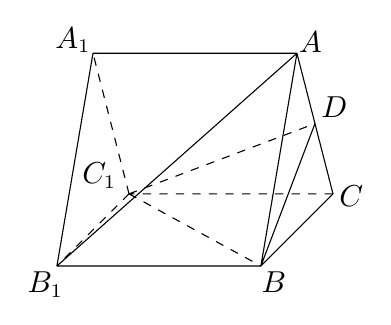
\begin{tikzpicture}[x=1pt, y=1pt,
    every node/.style={inner sep=0pt, font=\fontsize{10.5pt}{12.6pt}\selectfont}]
  \draw[line width=0.398pt] (86.405,77.303) -- (73.378,0.447) (99.432,26.501) -- (73.378,0.447) (12.701,77.303) -- (-0.326,0.447) (73.378,0.447) -- (-0.326,0.447) (86.405,77.303) -- (12.701,77.303) (92.919,51.902) -- (73.378,0.447) (86.405,77.303) -- (-0.326,0.447) (86.405,77.303) -- (99.432,26.501);
  \draw[line width=0.398pt, dash pattern=on 2.989pt off 2.989pt] (99.432,26.501) -- (25.728,26.501) (25.728,26.501) -- (12.701,77.303) (25.728,26.501) -- (-0.326,0.447) (25.728,26.501) -- (73.378,0.447) (25.728,26.501) -- (92.918,51.902);
  \node[anchor=center] at (5.500,82.000) {$A_1$};
  \node[anchor=center] at (91.340,81.380) {$A$};
  \node[anchor=center] at (-4.500,-6.200) {$B_1$};
  \node[anchor=center] at (78.050,-5.340) {$B$};
  \node[anchor=center] at (15.000,33.000) {$C_1$};
  \node[anchor=center] at (106.030,25.650) {$C$};
  \node[anchor=center] at (99.900,57.900) {$D$};
\end{tikzpicture}
%
% 【自验结果】逐路径照录；探针编译 0 警告。
